\let\negmedspace\undefined
\let\negthickspace\undefined
\documentclass[journal]{IEEEtran}
\usepackage[a5paper, margin=10mm, onecolumn]{geometry}
%\usepackage{lmodern} % Ensure lmodern is loaded for pdflatex
\usepackage{tfrupee} % Include tfrupee package

\setlength{\headheight}{1cm} % Set the height of the header box
\setlength{\headsep}{0mm}     % Set the distance between the header box and the top of the text

\usepackage{gvv-book}
\usepackage{gvv}
\usepackage{cite}
\usepackage{amsmath,amssymb,amsfonts,amsthm}
\usepackage{algorithmic}
\usepackage{graphicx}
\usepackage{textcomp}
\usepackage{xcolor}
\usepackage{txfonts}
\usepackage{listings}
\usepackage{enumitem}
\usepackage{mathtools}
\usepackage{gensymb}
\usepackage{comment}
\usepackage[breaklinks=true]{hyperref}
\usepackage{tkz-euclide}
\usepackage{multicol}
\usepackage{listings}
                                       
\def\inputGnumericTable{}                                 
\usepackage[latin1]{inputenc}                                
\usepackage{color}                                            
\usepackage{array}                                            
\usepackage{longtable}                                       
\usepackage{calc}                                             
\usepackage{multirow}                                         
\usepackage{hhline}
\usepackage{ifthen}                                           
\usepackage{lscape}
\usepackage{circuitikz}


\renewcommand{\thefigure}{\theenumi}
\renewcommand{\thetable}{\theenumi}
\setlength{\intextsep}{10pt} % Space between text and floats


\numberwithin{equation}{enumi}
\numberwithin{figure}{enumi}
\renewcommand{\thetable}{\theenumi}





\begin{document}
\bibliographystyle{IEEEtran}


\begin{center}
    \LARGE \textbf{GATE 2010 AG}\\[0.5em]
    \large \textbf{AI25BTECH11012 - UNNATHI GARIGE}
\end{center}

\textbf{Q.1 -- Q.25 carry one mark each.}
\bigskip
\begin{enumerate}


\item A particular solution of 
    \begin{align*}
      \frac{d^2 y}{dx^2} + 5 \frac{dy}{dx} - 3y = 6  
    \end{align*} is
    \hfill{\text{GATE AG 2010}}
\begin{multicols}{4}
\begin{enumerate}
    \item 2
    \item 0.5
    \item -0.5
    \item -2
\end{enumerate}
\end{multicols}


    \item The partial differential equation 
    \begin{align*}
    \frac{\partial^2 u}{\partial x^2} - 7 \frac{\partial^2 u}{\partial x \partial y} + 2 \frac{\partial^2 u}{\partial y^2} = 0
    \end{align*}
    is said to be
       \hfill{\text{GATE AG 2010}}
\begin{multicols}{4}
\begin{enumerate}
    \item parabolic
    \item hyperbolic
    \item elliptic
    \item eccentric
\end{enumerate}
\end{multicols}


    \item While carrying out tillage operations, negative slip is sometimes experienced with
    \begin{enumerate}
    \item  front wheels of two-wheel drive tractor \hfill{\text{GATE AG 2010}}
    \item  front wheels of four-wheel drive tractor 
    \item  front wheels of front wheel assisted tractor 
    \item  wheels of power tiller pulling a mould board plough
    \end{enumerate}


    \item A two-wheel drive tractor has a PTO speed of 540 rpm and it produces 35 kW net engine power. \\
    Corresponding torque available at PTO in N m will be \hfill{\text{GATE AG 2010}}
    \begin{multicols}{4}
    \begin{enumerate}
    \item 435--457
    \item 485--495
    \item 495--505
    \item 535--558
    \end{enumerate}
    \end{multicols}
    

    \item Raising the hitch on the implement frame of a pull type offset disk harrow without gauge wheel helps in  \hfill{\text{GATE AG 2010}}
    \begin{enumerate}
    \item  increasing the depth of penetration for the rear gang 
    \item increasing the depth of penetration for the front gang 
    \item decreasing the depth of penetration for the front gang 
    \item maintaining the same depth of penetration for both the gangs
    \end{enumerate}




    \item While deriving the Chezy formula for uniform flow, it is assumed that there is a balance between
     \hfill{\text{GATE AG 2010}}
    \begin{enumerate}
    \item gravity and inertial forces
    \item inertial and viscous forces
    \item frictional and gravity forces
    \item frictional and inertial forces
    \end{enumerate}



    \item A cross regulator is usually provided
    \hfill{\text{GATE AG 2010}}
    \begin{enumerate}
    \item at the head of the off-taking channel
    \item in the main channel upstream of the off-taking channel
    \item in the main channel downstream of the off-taking channel
    \item in the watercourse to regulate the outlets
    \end{enumerate}


   

    \item An effective rainfall of 20 mm h\(^{-1}\) occurs for 2 hours in a catchment. The time of concentration of the catchment is 1.5 hour. The peak of the resulting direct runoff hydrograph, in mm h\(^{-1}\), is
    \hfill{\text{GATE AG 2010}}
    \begin{multicols}{4}
    \begin{enumerate}
    \item 10
    \item 20
    \item 30
    \item 40
    \end{enumerate}
    \end{multicols}
    


\item The dimensionless number in heat transfer corresponding to Sherwood Number in mass transfer is 
\hfill{\text{GATE AG 2010}}
    \begin{multicols}{2}
    \begin{enumerate}
    \item Biot Number
    \item Schmidt Number
    \item Nusselt Number
    \item Graetz Number
    \end{enumerate}
    \end{multicols}


    
\item The interrelationship between thermal conductivity, dynamic viscosity and temperature of gas can be described as \hfill{\text{GATE AG 2010}}
\begin{enumerate}
   
\item  dynamic viscosity and thermal conductivity decrease as temperature increases 
\item  dynamic viscosity decreases and thermal conductivity increases as temperature increases 
\item dynamic viscosity and thermal conductivity decrease as temperature decreases 
\item  dynamic viscosity and thermal conductivity increase as temperature decreases 
\end{enumerate}

    
\item A system of equations represented as
\hfill{\text{GATE AG 2010}}
\begin{align*}
\myvec{
1 & -1 & 2 \\
2 & 1  & 4 \\
1 & 3  & 1
}
\myvec{
x_1 \\ x_2 \\ x_3
}
=
\myvec{
4 \\ y \\ 3
}
\end{align*}
is 

    \begin{multicols}{2}
    \begin{enumerate}
    \item consistent and has unique solution
    \item inconsistent and has no solution
    \item consistent and has infinite solutions
    \item inconsistent and has unique solution 
    \end{enumerate}
    \end{multicols}


    
\item There is a significant difference between scores from two groups if 

\begin{enumerate}
\item  the means are large compared to the standard error  \hfill{\text{GATE AG 2010}}
\item  the difference between the means is large compared to the standard error 
\item  the means are small compared to the standard error 
\item  the difference between the standard deviation is large compared to the means 
\end{enumerate}




\item The error in using trapezoidal rule for finding the value of
\begin{align*}
\int_0^1 \frac{dx}{1+x}    
\end{align*}
is \hfill{\text{GATE AG 2010}}
\begin{multicols}{4}
    \begin{enumerate}
    \item 0.0368
    \item 0.0468
    \item 0.0568
    \item 0.0668
    \end{enumerate}
    \end{multicols}


    
\item A farmer constructed a 2 m$^3$ 40 days HRT (hydraulic retention time) Deenbandhu model biogas plant. The gas will be solely used for cooking in a stove with a burner efficiency of 45\%. \\
If the density of biogas is 0.94 kg m$^{-3}$ with a heating value of 21 MJ kg$^{-1}$, the total effective energy available per day in MJ will be 
\hfill{\text{GATE AG 2010}}
\begin{multicols}{4}
    \begin{enumerate}
    \item 17.77
    \item 18.91
    \item 24.47
    \item 39.48
    \end{enumerate}
    \end{multicols}



    
\item A 2 $\times$ 0.3 m tractor drawn mould board plough while operating at a depth of 0.15 m has a draft of 2.5 kN at a forward speed of 3 km h$^{-1}$ with a field efficiency of 75\%. When the speed of operation is increased by 20\%, draft increased by 10\%. Assuming field efficiency, soil pulverization and soil inversion to be same at both the speeds, the performance index of the plough increases by 
\hfill{\text{GATE AG 2010}}
\begin{multicols}{4}
    \begin{enumerate}
    \item  0\%
    \item  9\%
    \item 20\%
    \item 30\%
    \end{enumerate}
    \end{multicols}



    
\item While evaluating a stationary power thresher for threshing wheat having a grain to straw ratio of 45\% and a moisture content (dry basis) of 14\%, the following observations were recorded for a duration of 5 min: \\
Quantity of grain (clean and broken) collected at main grain outlet = 16 kg, quantity of clean grain collected at bhusa outlet = 0.3 kg, quantity of clean grain obtained at sieve underflow and overflow = 0.2 kg and quantity of unthreshed grain from all outlets = 0.5 kg. \\
Percentage of blown and spilled grain are 
\hfill{\text{GATE AG 2010}}
\begin{multicols}{4}
    \begin{enumerate}
    \item  1.18, 3.03
    \item  1.25, 1.82
    \item  1.76, 1.18
    \item  1.88, 1.25 
    \end{enumerate}
    \end{multicols}





\item The Local Apparent Time (LAT) corresponding to 14 h 30' Indian Standard Time (IST) at a place in India (19$^\circ$ 07'N, 72$^\circ$ 51'E) in the month of April with a time correction of zero min will be
\hfill{\text{GATE AG 2010}}
\begin{multicols}{2}
    \begin{enumerate}
    \item  13 h 51' 24''
    \item  14 h 9' 39''
    \item  14 h 30'
    \item  15 h 8' 36''
    \end{enumerate}
    \end{multicols}




\item The following figure shows two advance curves for surface irrigation.
\begin{figure}[ht!]
    \centering
    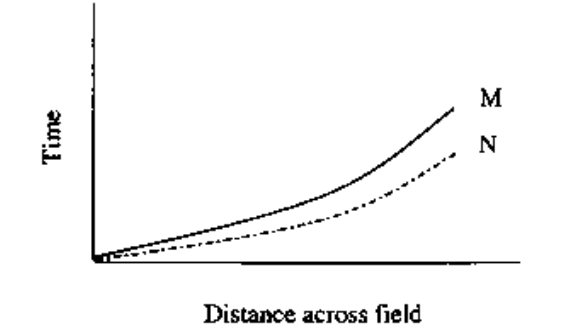
\includegraphics[width=0.4\textwidth]{ques_18.png}
    \caption{}
    \label{fig:proj31.jpeg}
\end{figure}
The advance represented by curve M is slower than N. This could be attributed to\\
P. the inflow rate to the field is lower\\
Q. the intake rate of the soil is lower\\
R. the field slope is flatter\\
S. the hydraulic roughness is greater for curve N than for curve M
\hfill{\text{GATE AG 2010}}
\begin{multicols}{2}
    \begin{enumerate}
    \item  P, Q
    \item  P, R
    \item  Q, S
    \item  R, S
    \end{enumerate}
    \end{multicols}



    
\item  A land survey is conducted on 40 m $\times$ 40 m grids and the elevations of grids in m from mean sea level are as follows.\\
\begin{center}
\begin{tabular}{|c|c|c|c|}
\hline
& A & B & C \\
\hline
1 & 102.3 & 103.0 & 103.7 \\
\hline
2 & 101.5 & 102.4 & 102.3 \\
\hline
3 & 101.2 & 103.5 & 102.6 \\
\hline
\end{tabular}
\end{center}
Assuming that cut is equal to fill, the volume of earthwork required to level the area in m$^3$ is
\hfill{\text{GATE AG 2010}}
\begin{multicols}{4}
    \begin{enumerate}
    \item  4480
    \item  4840 
    \item  5480
    \item  6480
    \end{enumerate}
    \end{multicols}

    
\item For hydrologic design, the entire runoff hydrograph should be known in case of
\begin{enumerate}
    \item Drop spillway   \hfill{\text{GATE AG 2010}}
    \item Chute spillway
    \item Drop inlet spillway
    \item Ogee spillway
    \end{enumerate}


    
\item  For a given watershed, the rainfall erosivity index is 1000 MJ mm ha$^{-1}$ h$^{-1}$ year$^{-1}$, soil erodibility index is 0.25 Mg h ha$^{-1}$ MJ$^{-1}$ mm$^{-1}$, crop management factor is 0.75, conservation practice factor is 1.0 and slope length factor is 0.2. If by certain conservation practices, the conservation practice factor is reduced to 0.7, then the reduction in soil loss, in Mg ha$^{-1}$ year$^{-1}$ is
\hfill{\text{GATE AG 2010}}
\begin{multicols}{4}
    \begin{enumerate}
    \item  9.75
    \item  11.25
    \item  11.75
    \item  12.25
    \end{enumerate}
    \end{multicols}

 

  \item Eight log cycle reduction of \textit{Clostridium botulinum} having z-value of $9^{\circ}\mathrm{C}$ needs a process time of 1.5 minute at $121^{\circ}\mathrm{C}$ temperature. The same degree of reduction at $130^{\circ}\mathrm{C}$ temperature will require a process time of
  \hfill{\text{GATE AG 2010}}
\begin{multicols}{4}
    \begin{enumerate}
    \item  72 s 
    \item  54 s
    \item  18 s
    \item  9 s
    \end{enumerate}
    \end{multicols}
  
   

    \item Let $m$, $n$ and $p$ be the numbers of carbon, hydrogen, and fluorine atoms in a refrigerant. The identification number of the refrigerant is
     \hfill{\text{GATE AG 2010}}
\begin{multicols}{4}
    \begin{enumerate}
    \item $R(m+1)(n-1)p$
    \item  $R(m-1)(n+1)p$
    \item $R(m-1)(n-1)p$
    \item  $R(m+1)(n+1)p$
    \end{enumerate}
    \end{multicols}


     
    \item A household refrigerator of 1 TR capacity operates half the time during 13-hour long days and 30\% time during the nights.\\
    If coefficient of performance is 4.7 then at Rs. 3 per kWh, monthly (30 days) electricity bill in Rupees for the refrigerator is
      \hfill{\text{GATE AG 2010}}
\begin{multicols}{4}
    \begin{enumerate}
    \item 110
    \item 220
    \item 440
    \item 660
    \end{enumerate}
    \end{multicols}

    

    \item Air at $40^\circ$C temperature has partial vapour pressure of 2.4 kPa. If universal gas constant is $8.314$ kJ kg$^{-1}$ K$^{-1}$ and total pressure is $101.325$ kPa then humid volume of air in m\textsuperscript{3}/(kg dry air) is
      \hfill{\text{GATE AG 2010}}
\begin{multicols}{4}
    \begin{enumerate}
    \item 0.809
    \item 0.908
    \item 1.089
    \item 1.098
    \end{enumerate}
    \end{multicols}
      


\textbf{Q.26 -- Q.55 carry two marks each.}

\vspace{0.5cm}
    \item The curl of the vector $A = xyi + yzj + zxk$ ($i, j, k$ represent unit vectors along the three orthogonal axes) is
     \hfill{\text{GATE AG 2010}}
\begin{multicols}{4}
    \begin{enumerate}
    \item $xyi + yj + zk$
    \item $-xi - yj - zk$
    \item $yi + zj + xk$
    \item  $-yi - zj - xk$
    \end{enumerate}
    \end{multicols}
      
  

    \item The angle of intersection between the planes $x - 3y + 2z = 10$ and $2x + 4y + 5z = 0$ is
    \hfill{\text{GATE AG 2010}}
\begin{multicols}{4}
    \begin{enumerate}
    \item $30^\circ$
    \item $60^\circ$
    \item $75^\circ$
    \item $90^\circ$
    \end{enumerate}
    \end{multicols}
      

       
    \item The Laplace transformation of $t^2 e^{4t}$ is
    \hfill{\text{GATE AG 2010}}
\begin{multicols}{4}
    \begin{enumerate}
    \item $\frac{4!}{(s-4)^4}$
    \item $\frac{3!}{(s-4)^4}$
    \item $\frac{3!}{(s-4)^3}$
    \item $\frac{4!}{(s-4)^3}$
    \end{enumerate}
    \end{multicols}
  

    
    \item The derivative of 
    \begin{align*}
        y = \sqrt{x + \sqrt{x + \sqrt{x + \cdots}}}
    \end{align*}
        with respect to x at y=0 is
    \hfill{\text{GATE AG 2010}}
\begin{multicols}{4}
    \begin{enumerate}
    \item -1
    \item 0
    \item 1
    \item 2
    \end{enumerate}
    \end{multicols}
  


    \item The value of \begin{align*}\int_0^2 \int_0^x xy \, dx \, dy\end{align*} is
     \hfill{\text{GATE AG 2010}}
\begin{multicols}{4}
    \begin{enumerate}
    \item 0.5
    \item 1
    \item 2
    \item 4
    \end{enumerate}
    \end{multicols}  



 
    \item A thresher requires a torque of $(5000 + 500 \sin{\alpha})$ Nm to drive, where $\alpha$ is the angle of rotation of shaft measured from certain datum. The thresher is directly coupled to an engine which produces a torque of $(5000 + 600 \sin{2\alpha})$ Nm. The flywheel and the rotary parts attached to the engine have a mass of $500\,\text{kg}$ at a radius of gyration $0.4\, \text{m}$. The maximum angular acceleration of the flywheel in rad sec$^{-2}$ will be
       \hfill{\text{GATE AG 2010}}
\begin{multicols}{4}
    \begin{enumerate}
    \item $3.46$
    \item $5.46$
    \item $7.46$
    \item $9.46$  
    \end{enumerate}
    \end{multicols}  
  


   \item The tractor seat vibrates with a frequency of 1~Hz when there is no damping. When damping is provided, the frequency of damped vibration is reduced by 10\%. The damping factor is
    \hfill{\text{GATE AG 2010}}
\begin{multicols}{4}
    \begin{enumerate}
    \item $0.21$
    \item $ 0.39$
    \item $0.44$
    \item $0.93$  
    \end{enumerate}
    \end{multicols}  
   


    \item A disk type mower, operated by a tractor PTO, has six discs with a swath of 0.4~m per disk. The specific energy required for cutting is 2.1~kJ~m$^{-2}$ and specific power losses due to air, stubble and gear train friction are 2~kW~m$^{-1}$ of cutting width. If the mower with tractor requires a propelling force of 2~kN, the total power requirement for carrying out mowing in kW at a forward speed of 3~km~h$^{-1}$
     \hfill{\text{GATE AG 2010}}
\begin{multicols}{4}
    \begin{enumerate}
    \item  6.47 
    \item 7.57
    \item 8.33
    \item 10.67
    \end{enumerate}
    \end{multicols}  
    


    \item In a tractor differential, the pinion on the propeller shaft has 12 teeth and the crown gear has 60 teeth. The propeller shaft rotates at 1000~rpm and the right rear axle rotates at 210~rpm while taking a left turn. The rotation of the left rear axle in rpm will be
      \hfill{\text{GATE AG 2010}}
\begin{multicols}{4}
    \begin{enumerate}
    \item 170
    \item 180
    \item 190
    \item 200
    \end{enumerate}
    \end{multicols}  
    


    \item Match all items in Group I with correct options from those in Group II

    \textbf{Group I}\hspace{4cm}\textbf{Group II}\\
    i. Slider crank mechanism \hspace{1.75cm} a. Tractor steering\\
    ii. Four bar linkage mechanism \hspace{1cm} b. Attachment of pitman to knife head\\
    iii. Ball and socket joint \hspace{2cm} c. Planting unit of rice transplanter\\
    iv. Worm and roller type unit \hspace{1.25cm} d. Vertical conveyor reaper
     \hfill{\text{GATE AG 2010}}
\begin{multicols}{2}
    \begin{enumerate}
    \item i-d, ii-c, iii-b, iv-a
    \item i-b, ii-c, iii-a, iv-d
    \item i-c, ii-a, iii-d, iv-b
    \item i-b, ii-c, iii-a, iv-d
    \end{enumerate}
    \end{multicols}  
    
   

    \item The mass of a 3.0~mm crumbled soil thread is \(17.5 \times 10^{-3}\)~kg. On oven-drying, the mass of the soil thread reduces to \(14.9 \times 10^{-3}\)~kg. The liquid limit of the soil sample is 35.4\%. The plasticity index of the soil sample is
     \hfill{\text{GATE AG 2010}}
\begin{multicols}{4}
    \begin{enumerate}
    \item 14.9 
    \item 18.0
    \item 32.8
    \item 35.4
    \end{enumerate}
    \end{multicols}  
    

    
    \item A pipeline carrying a discharge of 500 litres per minute branches into two parallel pipes, X and Y, as shown in the following figure. The length and diameter of pipes X and Y are shown in the figure.  \hfill{\text{GATE AG 2010}}
\begin{figure}[ht!]
    \centering
    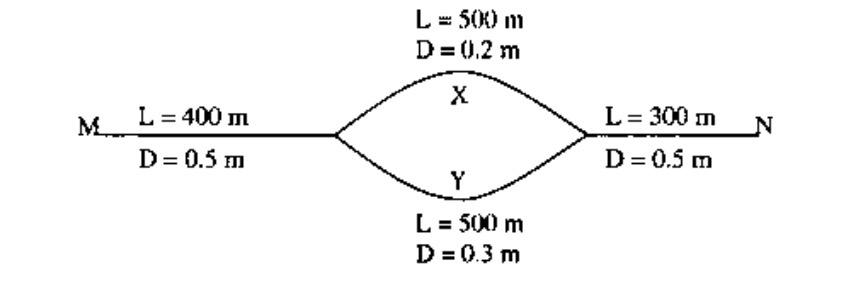
\includegraphics[width=0.7\textwidth]{ques_37.jpeg}
    \caption{}
    \label{fig:proj32.jpeg}
\end{figure}

The friction factor, \(f\), for all pipes is 0.030. The ratio of flow in pipes X and Y is
      
\begin{multicols}{4}
    \begin{enumerate}
    \item 0.36 
    \item 0.44
    \item 0.67 
    \item 1.00
    \end{enumerate}
    \end{multicols}  

    
    \item A pump installed in an existing irrigation system delivers 3200 litres per minute flow at a total head of 60.0~m. The impeller diameter is 0.26~m and it is rotated at 1800~rpm. A motor with an output shaft power of 54~kW is required to drive the pump. The existing irrigation system, however, is modified in such a way that the discharge pressure requirement is reduced to 52.0~m while keeping the flow rate unchanged. If the existing pump is to be utilized, then to meet the new system requirement, the impeller diameter in m will be
     \hfill{\text{GATE AG 2010}}
\begin{multicols}{4}
    \begin{enumerate}
    \item 0.24
    \item 0.25
    \item  0.26
    \item  0.27
    \end{enumerate}
    \end{multicols}  



% Q39
\item
In order to evaluate irrigation distribution, an irrigator estimates the depth of infiltration, in mm, around a field as given below.
\[
\begin{array}{cccc}
42 & 36 & 32 & 38 \\
40 & 32 & 35 & 34 \\
36 & 30 & 27 & 31 \\
45 & 38 & 34 & 44 \\
\end{array}
\]
The distribution uniformity for the irrigation is
\hfill{\text{GATE AG 2010}}
\begin{multicols}{4}
    \begin{enumerate}
    \item 80.4
    \item 81.9 
    \item 87.9
    \item 88.1
    \end{enumerate}
    \end{multicols}  




% Q40
\item
A parabolic shaped grassed waterway has a top width of 4 m, a maximum depth of 0.40 m, and a slope of 2.5\%. The Manning's 'n' value is 0.035, and there is no provision of freeboard. \\
The discharge carrying capacity of the waterway in m$^3$\,s$^{-1}$ is
\hfill{\text{GATE AG 2010}}
\begin{multicols}{4}
    \begin{enumerate}
    \item 1.38
    \item 1.52
    \item 1.76
    \item 1.96
    \end{enumerate}
    \end{multicols}  





% Q41
\item
In an irrigation command area, the irrigation interval, gross application in an irrigation and the application efficiency are 20 days, 75 mm and 60\%, respectively. The soil is homogeneous with $K=0.9$ m day$^{-1}$. The impermeable layer is at a depth of 7 m from the ground surface. The area is to be tile drained with tiles at a depth of 2 m below the ground surface. The maximum permissible steady state water table height mid-way between the drains, from the plane of the drain, is 1.2 m. Using the steady state approach of Hooghoudt, assuming an equivalent depth of 4.12 m, the drain spacing in m will be
\hfill{\text{GATE AG 2010}}
\begin{multicols}{2}
    \begin{enumerate}
    \item 115.25
    \item 131.75
    \item 146.25
    \item 186.35
    \end{enumerate}
    \end{multicols}  

    
% Q42
\item
A tubewell in a confined aquifer has a diameter of 0.30 m. For a certain yield, the radius of influence is 400 m. All conditions remaining the same, if the diameter of the well is doubled, then the percentage increase in the yield is
\hfill{\text{GATE AG 2010}}
\begin{multicols}{4}
    \begin{enumerate}
    \item 9.28
    \item 9.63
    \item 10.00
    \item 10.23
    \end{enumerate}
    \end{multicols}  


    
% Q43
\item
The heating surface of an oven has an emissivity of 0.7 with 0.1 m$^2$ surface area and is maintained at 280$^\circ$C. The view factor of this surface with respect to a piece of bread of 0.01 m$^2$ surface area is 0.05. If bread has emissivity of 0.3 and receives 10 W of energy through radiation from the heating surface (with Stephan-Boltzmann constant of $5.67 \times 10^{-8}$ W m$^{-2}$ K$^{-4}$), the steady state bread surface temperature in $^\circ$C is
\hfill{\text{GATE AG 2010}}
\begin{multicols}{4}
    \begin{enumerate}
    \item 137.2
    \item 118.5
    \item 97.3
    \item 84.5
    \end{enumerate}
    \end{multicols}  


    
% Q44
\item
In parboiling operation water to paddy ratio is 1.2. Water of specific heat capacity of 4.2 kJ kg$^{-1}$ K$^{-1}$ is heated from 25$^\circ$C to 85$^\circ$C by condensation of steam supplying 2114 kJ kg$^{-1}$ latent heat across a tubular heat exchanger. When 1 ton paddy at 30$^\circ$C is poured into the hot water the mixture temperature stabilizes at 75$^\circ$C. Assuming no heat loss to the surrounding this implies:
\\
P. steam supplied is 431 kg \\
Q. specific heat capacity of paddy is 1.12 kJ kg$^{-1}$ K$^{-1}$ \\
R. steam supplied is 143 kg \\
S. specific heat capacity of paddy is 2.11 kJ kg$^{-1}$ K$^{-1}$
\hfill{\text{GATE AG 2010}}
\begin{multicols}{4}
    \begin{enumerate}
    \item P,Q
    \item Q,R
    \item R,S
    \item  P,S
    \end{enumerate}
    \end{multicols}  



\item Density, specific heat capacity and thermal conductivity of air are $0.99~\text{kg}\text{m}^{-3},~1\text{kJ}\text{kg}^{-1}\text{K}^{-1}$ and $0.03~\text{W}\text{m}^{-1}\text{K}^{-1}$ respectively. Convective heat transfer coefficient of air medium and equimolar counter-diffusion mass transfer coefficient of water vapour into air are $35~\text{W}\text{m}^{-2}\text{K}^{-1}$ and $0.032~\text{m}^{2}\text{s}^{-1}$ respectively. The mass diffusivity of water vapour into the air in $\text{m}^2\text{s}^{-1}$ is 
\hfill{\text{GATE AG 2010}}
\begin{multicols}{4}
    \begin{enumerate}
    \item $2.46 \times 10^{-5}$
    \item $4.62 \times 10^{-5}$
    \item $8.25 \times 10^{-4}$
    \item  $2.85 \times 10^{-5}$
    \end{enumerate}
    \end{multicols}  




\item 20\% sucrose solution is boiled and frozen separately.\\
If latent heat of vaporization at $100^\circ$C and the latent heat of crystallization at $0^\circ$C are 2257 and 334 kJ kg$^{-1}$, respectively, then the ratio of freezing point depression to boiling point elevation is 
\hfill{\text{GATE AG 2010}}
\begin{multicols}{4}
    \begin{enumerate}
    \item 4.2
    \item 2.3 
    \item 3.6
    \item 2.4
    \end{enumerate}
    \end{multicols}  




\item Carrot slices of 2 mm thickness are freeze dried from initial free moisture content of 80\% (wet basis) to a final free moisture content of 2\% (wet basis). Mass density of fresh carrot is $1100~\text{kg}\text{m}^{-3}$. Thermal conductivity of dried layer is $0.005\text{W}\text{m}^{-1}\text{K}^{-1}$. Latent heat of sublimation at $-35^\circ$C is $2840~\text{kJ}~\text{kg}^{-1}$ and product surface temperature is $-5^\circ$C. The total drying time in hour is
\hfill{\text{GATE AG 2010}}
\begin{multicols}{4}
    \begin{enumerate}
    \item 1.2
    \item 2.3
    \item  3.2
    \item 5.4
    \end{enumerate}
    \end{multicols}  




\textbf{Common Data Questions}

\textbf{Common Data for Questions 48 and 49:}
\vspace{0.5cm} \newline
A field sprayer having 16 fan type spray nozzles spaced 0.5 m apart is moving at a forward speed of 3.5 km/hr with an application rate of 1 m$^3$ ha$^{-1}$. At a deposition level 430 mm below the tip of the nozzle, the discharge rate across a 0.2 m width at the centre of the sprayed tip is essentially constant at 15 ml min$^{-1}$ per 10 mm of lateral distance. On each side of this 0.2 cm centre strip, the discharge rate per mm of width decreases uniformly to zero at a lateral distance of 0.36 m from the nozzle centre line.

\item  The discharge rate per nozzle in m$^3$ h$^{-1}$ will be
\hfill{\text{GATE AG 2010}}
\begin{multicols}{4}
    \begin{enumerate}
    \item 0.175   
    \item  0.350
    \item 0.215
    \item 0.430
    \end{enumerate}
    \end{multicols}  



\item  The nozzle tip height in mm above the deposition level that would give uniform coverage will be  
\hfill{\text{GATE AG 2010}}
\begin{multicols}{4}
    \begin{enumerate}
    \item 602
    \item  546 
    \item 501
    \item 477
    \end{enumerate}
    \end{multicols}  




\textbf{Common Data for Questions 50 and 51:}

In a drying experiment on potato slices of 5 mm thickness the initial moisture content of 4.2 kg water (kg dry matter)$^{-1}$ got reduced to 0.03 kg water (kg dry matter)$^{-1}$ by the application of hot air at $65^\circ$C having absolute humidity of 0.02 kg water vapour (kg dry air)$^{-1}$ with saturation water vapour pressure of 6 kPa. Critical moisture content of 2.5 kg water (kg dry matter)$^{-1}$ was reached after 3 hour of drying time. The dry matter concentration in the drying chamber was 5 kg per m$^2$ of surface area.
\vspace{0.125cm}
\item  The mass transfer coefficient in kg mole m$^{-2}$ s$^{-1}$ during drying is\\ 
. \hfill{\text{GATE AG 2010}}
\begin{multicols}{4}
    \begin{enumerate}
    \item $1.43 \times 10^{-7}$
    \item $3.14 \times 10^{-3}$
    \item $4.31 \times 10^{-5}$
    \item $7.87 \times 10^{-8}$
    \end{enumerate}
    \end{multicols}  




\item  Mass diffusivity of water vapour in m$^2$ s$^{-1}$ during the falling rate phase of drying is 
. \hfill{\text{GATE AG 2010}}
\begin{multicols}{4}
    \begin{enumerate}
    \item $7.01 \times 10^{-4}$ 
    \item $5.07 \times 10^{-4}$
    \item  $3.71 \times 10^{-5}$
    \item $1.07 \times 10^{-3}$
    \end{enumerate}
    \end{multicols}  


\large{\textbf {Linked Answer Questions}}

\textbf{Statement for Linked Answer Questions 52 and 53:}

A 37\,kW two-wheel drive tractor weighing 20\,kN with a wheel base of 2.1\,m is having the option to be fitted with either 12.4--28 12PR or 13.6--28 12 PR at the rear axle. The ratio of section height and section width for all tyres is 0.75. On a level ground, the weight distribution on the front and rear axles is 35 and 65\% of the total tractor weight, respectively. Cone index of soil is 1200\,kPa.
\vspace{0.25cm}


    \item The motion resistance ratio of each of the rear wheels when fitted with the above-mentioned tyres at normal tyre inflation pressure while moving on a level ground will be
    \hfill{\text{GATE AG 2010}}
\begin{multicols}{4}
    \begin{enumerate}
    \item 0.04, 0.04
    \item 0.047, 0.055
    \item 0.051, 0.049
    \item 0.057
    \end{enumerate}
    \end{multicols}  




    \item Net traction developed in kN by the rear wheels when fitted with 13.6--28 12 PR tyre at normal inflation pressure on a level ground with 15\% wheel slip will be
     \hfill{\text{GATE AG 2010}}
\begin{multicols}{4}
    \begin{enumerate}
    \item  8.79
    \item 9.18
    \item 9.78
    \item 10.32
    \end{enumerate}
    \end{multicols}  



\textbf{Statement for Linked Answer Questions 54 and 55:}
\vspace{0.25cm}

The peak of a flood hydrograph due to a 1--h duration isolated storm in a catchment of area 13.5\,km$^2$ is 135\,m$^3$s$^{-1}$. The total depth of rainfall is 54\,mm. Assume a constant base flow of 10\,m$^3$s$^{-1}$ and phi--index equal to 4\,mm\,h$^{-1}$.


    \item The peak of 1--h unit hydrograph for the catchment in m$^3$s$^{-1}$ is
    \hfill{\text{GATE AG 2010}}
\begin{multicols}{4}
    \begin{enumerate}
    \item 15
    \item 20
    \item 25
    \item 30
    \end{enumerate}
    \end{multicols}  




    \item Assuming the above 1--h unit hydrograph to be triangular in shape with the time to peak as t hour, the peak of the 2--h unit hydrograph for the catchment in m$^3$s$^{-1}$ is
   \item The peak of 1--h unit hydrograph for the catchment in m$^3$s$^{-1}$ is
    \hfill{\text{GATE AG 2010}}
\begin{multicols}{4}
    \begin{enumerate}
    \item  13.25 
    \item 18.75
    \item 21.25
    \item 26.75
    \end{enumerate}
    \end{multicols}    





\large{\textbf{General Aptitude (GA) Questions}}

\textbf{Q.56 -- Q.60 carry one mark each.}
\vspace{0.25cm}

% Q.56
\item Choose the most appropriate word from the options given below to complete the following sentence:

\textbf{His rather casual remarks on politics \underline{\hspace{2cm}} his lack of seriousness about the subject.}
 \hfill{\text{GATE AG 2010}}
    \begin{enumerate}
     \item masked
    \item belied
    \item betrayed
    \item suppressed
\end{enumerate}



% Q.57
\item Which of the following options is the closest in meaning to the word below:\\
\textbf{Circumlocutous}
\hfill{\text{GATE AG 2010}}
    \begin{enumerate}
     \item cyclic
    \item indirect
    \item confusing
    \item crooked
    \end{enumerate}



\item Choose the most appropriate word from the options given below to complete the following sentence:
\textbf{If we manage to \underline{\hspace{2cm}} our natural resources, we would leave a better planet for our children.}

\begin{enumerate}
    \item uphold
    \item restrain
    \item cherish
    \item conserve
\end{enumerate}



% Q.59
\item 25 persons are in a room. 15 of them play hockey, 17 of them play football and 10 of them play both hockey and football. Then the number of persons playing neither hockey nor football is:
 \hfill{\text{GATE AG 2010}}
\begin{multicols}{4}
    \begin{enumerate}
    \item 2
    \item 17
    \item 13
    \item 3
    \end{enumerate}
    \end{multicols}    






% Q.60
\item The question below consists of a pair of related words followed by four pairs of words. Select the pair that best expresses the relation in the original pair.

\textbf{Unemployed : Worker}

\begin{enumerate}
    \item fallow : land
    \item unaware : sleeper
    \item wit : jester
    \item renovated : house
\end{enumerate}



\vspace{0.5cm}

\textbf{Q.61 -- Q.65 carry two marks each.}
\vspace{0.5cm}

\item If $137 + 276 = 435$ how much is $731 + 672$?
\hfill{\text{GATE AG 2010}}
\begin{multicols}{4}
    \begin{enumerate}
    \item 534
    \item 1403
    \item 1623
    \item 1513
    \end{enumerate}
    \end{multicols}    




\item Hari (H), Gita (G), Irfan (I) and Saira (S) are siblings (i.e. brothers and sisters). All were born on 1\textsuperscript{st} January. The age difference between any two successive siblings (that is born one after another) is less than 3 years. Given the following facts:\\
\begin{enumerate}
    \item Hari's age + Gita's age $>$ Irfan's age + Saira's age.
    \item The age difference between Gita and Saira is 1 year. However, Gita is not the oldest and Saira is not the youngest.
    \item There are no twins.
\end{enumerate}
In what order were they born (oldest first)?
\hfill{\text{GATE AG 2010}}
\begin{multicols}{4}
    \begin{enumerate}
    \item  HSGI
    \item  SGHI
    \item IGSH
    \item IHSG
    \end{enumerate}
    \end{multicols}    



 
\item \textbf{Modern warfare has changed from large scale clashes of armies to suppression of civilian populations. Chemical agents that do their work silently appear to be suited to such warfare; and regretfully, there exist people in military establishments who think that chemical agents are useful tools for their cause.}

\textit{Which of the following statements best sums up the meaning of the above passage:}
\hfill{\text{GATE AG 2010}}
\begin{enumerate}
 
\item  Modern warfare has resulted in civil strife.
\item Chemical agents are useful in modern warfare.
\item  Use of chemical agents in warfare would be undesirable.
\item  People in military establishments like to use chemical agents in war.
\end{enumerate}



\item 5 skilled workers can build a wall in 20 days; 8 semi-skilled workers can build a wall in 25 days; 10 unskilled workers can build a wall in 30 days. If a team has 2 skilled, 6 semi-skilled and 5 unskilled workers, how long will it take to build the wall?
\hfill{\text{GATE AG 2010}}
\begin{multicols}{4}
    \begin{enumerate}
    \item  20 days 
    \item  18 days
    \item 16 days
    \item  15 days
    \end{enumerate}
    \end{multicols}    



\item Given digits 2, 2, 3, 3, 3, 4, 4, 4, 4 how many distinct 4 digit numbers greater than 3000 can be formed?
\hfill{\text{GATE AG 2010}}
\begin{multicols}{4}
    \begin{enumerate}
    \item  50 
    \item   51
    \item 52
    \item  54
    \end{enumerate}
    \end{multicols}    



\begin{center}
    \textbf{END OF THE QUESTION PAPER}
\end{center}
   






\end{enumerate}




















\end{document}
